\documentclass[9pt,twocolumn,twoside,lineno]{pnas-new}
% Use the lineno option to display guide line numbers if required.

\usepackage{xr}
\usepackage{graphicx}
\usepackage{subcaption}

%----Helper code for dealing with external references----
% (by cyberSingularity at http://tex.stackexchange.com/a/69832/226)


\makeatletter

\newcommand*{\addFileDependency}[1]{% argument=file name and extension
\typeout{(#1)}% latexmk will find this if $recorder=0
% however, in that case, it will ignore #1 if it is a .aux or 
% .pdf file etc and it exists! If it doesn't exist, it will appear 
% in the list of dependents regardless)
%
% Write the following if you want it to appear in \listfiles 
% --- although not really necessary and latexmk doesn't use this
%
\@addtofilelist{#1}
%
% latexmk will find this message if #1 doesn't exist (yet)
\IfFileExists{#1}{}{\typeout{No file #1.}}
}\makeatother

\newcommand*{\myexternaldocument}[1]{%
\externaldocument{#1}%
\addFileDependency{#1.tex}%
\addFileDependency{#1.aux}%
}
%------------End of helper code--------------

% put all the external documents here!
\myexternaldocument{SI}



\templatetype{pnasresearcharticle}

\title{Collective Memory of Dynamic Events: Analyzing Persistence of Attention to Bankruptcy Events}

% Use letters for affiliations, numbers to show equal authorship (if applicable) and to indicate the corresponding author
\author[a,b,c,1]{Kathleen M. Jagodnik}
\author[a,b]{Sharon Dekel}
\author[c]{Alon Bartal} 

\affil[a] {Department of Psychiatry, Harvard Medical School, Boston, Massachusetts, USA}

\affil[b] {Department of Psychiatry, Massachusetts General Hospital, Boston, Massachusetts, USA}

\affil[c] {The School of Business Administration, Bar-Ilan University, Ramat Gan, 5290002, Israel}


% Please give the surname of the lead author for the running footer
\leadauthor{Jagodnik} 

% Please add a significance statement to explain the relevance of your work
\significancestatement{Little is known about the persistence of collective memory of dynamic events.
Previous research analyzed collective memory of discrete events that do not change after occurring (e.g., celebrity deaths).
Extending that research, we analyzed collective memory of U.S. companies that declared Chapter 11 bankruptcy, involving dynamic, persistent post-bankruptcy company status.
Analyzing Twitter posts mentioning companies before and after bankruptcy announcement, we observe intense attention following the announcement, with varying levels of memory persistence.
Assessing systematic differences in how bankrupt companies persist in memory, we successfully predicted the post-bankruptcy persistence level based on pre-bankruptcy user posting behavior. 
We emphasize the impact of pre-bankruptcy attention on how a company remains in public attention, offering valuable insights for financial and media stakeholders.
}

% Please include corresponding author, author contribution and author declaration information
\authorcontributions{K.M.J.: Designed research; Collected and analyzed data; Wrote and revised the paper. S.D.: Wrote and revised the paper. A.B.: Designed research; Performed research; Collected and analyzed data; Wrote and revised the paper.}
\authordeclaration{All authors declare no competing interests.}
%\equalauthors{\textsuperscript{1}A.O.(Author One) contributed equally to this work with A.T. (Author Two) (remove if not applicable).}
\correspondingauthor{\textsuperscript{1}Corresponding author E-mail: kjagodnik@mgh.harvard.edu}

% At least three keywords are required at submission. Please provide three to five keywords, separated by the pipe symbol.
\keywords{bankruptcy $|$ collective memory $|$  dynamic events $|$ public attention $|$ social media}


%%%%%%%%%%%%%%%%%%%%%%%%%%%%%% abstract %%%%%%%%%%%%%%%%%%%%%%%%%%%%%%
\begin{abstract}
Collective attention and memory involving significant events have been quantitatively studied using large-scale social media data. 
Previous studies analyzed user attention to discrete events that do not change post-event (e.g., a celebrity's death), and assume universal public attention patterns.
However, many significant events are dynamic, involving ongoing updates. 
Additionally, individuals may exhibit different attention patterns.
We investigate collective memory of U.S. companies that filed for Chapter 11 bankruptcy and were mentioned on Twitter.
Unlike discrete events, a company's financial status under Chapter 11 bankruptcy is dynamic, as the company typically remains operational.
These continuous updates can affect public attention over time following bankruptcy events.
We collected 248,936 Twitter mentions of 74 companies one month before and after each bankruptcy event.
We observed a sharp spike in attention after bankruptcy, and identified Low or High persistence level of attention compared with attention level prior to bankruptcy.
We fit two bi-exponential models to the tweeting patterns of Low and High attention levels.
Importantly, we successfully (F1-score of 0.81) predicted the post-bankruptcy persistence level of public attention as of the day of bankruptcy.
Studying bankruptcy events via social media coverage reveals varying attention patterns, informs how pre-bankruptcy attention shapes the remembrance of a company post-bankruptcy, and offers novel insights involving collective memory of dynamic events.
\end{abstract}

\dates{This manuscript was compiled on \today}
\doi{\url{www.pnas.org/cgi/doi/10.1073/pnas.XXXXXXXXXX}}

\begin{document}

\maketitle
\thispagestyle{firststyle}
\ifthenelse{\boolean{shortarticle}}{\ifthenelse{\boolean{singlecolumn}}{\abscontentformatted}{\abscontent}}{}

%Note: please start your introduction without including the word ``Introduction'' as a section heading (except for math articles in the Physical Sciences section); this heading is implied in the first paragraphs. 


%===============================================================
%  Introduction
%===============================================================

% ----- Remember and Forget Financial Events ---------------
%\firstpage{7}
\dropcap{C}ollective memory involves significant events shared by social groups \cite{halbwachs1992collective}.
It can be modeled as communicative (individual-level communications) and cultural (societal activities such as rites and monuments) forms of memory \cite{assmann1995collective, candia2019universal}.

Psychologists have studied top-down and bottom-up approaches to memory formation and retention. 
Top-down approaches examine how familiarity, narrative templates, and cultural attractors such as children's songs \cite{rubin1995memory} contribute to the persistence of collective memory \cite{rubin1995memory,buskell2017cultural,roediger2016recognizing}.
Bottom-up approaches largely focus on retrieval-induced forgetting and the mnemonic power of social affinities \cite{hirst2018collective, coman2015social}.

Computational social scientists have studied the expression of collective memory via  attention to cultural products by, for example, measuring the number of discussions on movies, songs, number of page views on Wikipedia, and citations of academic papers \cite{yu2016pantheon, candia2019universal, west2021postmortem, jara2019medium, higham2017fame}. 
These measures do not directly capture collective memory; they serve as indicators of public attention spillovers that often result in online searches and discussions \cite{candia2019universal}.
Cultural products initially receive high attention close to their release (communicative memory), which diminishes over time to cultural memory level \cite{west2021postmortem, candia2019universal}.
In simple words, when a cultural product becomes popular, people widely talk about it (high attention).
This heightened interest makes individuals more likely to remember a product.
When a cultural product moves away from communicative memory, it loses this intense attention.
Hence, attention has a vital role in the formation and dissemination of collective memory \cite{candia2019universal}.
The computational approach aligns closely with Jan Assmann's \cite{assmann2011communicative} definition of collective memory, which focuses on the cultural products remembered by communities or groups of people.
We follow the computational social science approach to study collective  memories of significant events by analyzing cultural consumption of information expressed by attention. 

Memories of significant events often vary between individuals \cite{mena2016forgetting}. 
Analyzing significant corporate irresponsibility events (e.g., bankruptcy) showed that some events do not persist in collective memory \cite{crane2013modern,fig2005manufacturing}.
For example, the scandal of HealthSouth's CEO inflating profits by 1.4B USD  \cite{goodman2003rebranding} and Volkswagen's emissions tests fraud were collectively forgotten \cite{tuttle2015volkswagen}.
In contrast, Nike's child labor use, and Enron's fraudulent accounting, persist in collective memory \cite{mena2016forgetting}.

% ----- Memory Manipulation by the Company ---------------
% User Attention to Events
Persistence of corporate irresponsibility events in collective memory can result from natural inertia or actions designed to achieve an agenda (i.e., strategy) \cite{fine2012sticky}.
Some companies apply strategies to modify or erase the persistence of negative events from collective memory \cite{fine2012sticky, brockmeier2002remembering}.
%Regardless of strategies, collective memory and attention usually do not persist for prolonged periods \cite{igarashi2022two,candia2019universal}.

% Short-Term Manipulation
In the short term, companies can apply strategies to shape the collective memory of an event by addressing the harm caused; influencing media attention; and attributing blame either by accepting, denying, or shifting responsibility \cite{zadek2004civil, mcdonnell2013keeping, storm2012durability}.
Indeed, firms heavily invest in their media representation strategy \cite{desai2014impact}.
For example, the Talvivaara mining company tried to reduce the persistence in collective memory of the ecological disaster it caused in Finland by shifting media attention \cite{mena2016forgetting}.
The company argued that news of the disaster obscured the mine's economic benefits and job creation \cite{mena2016forgetting}.

% Long-term Manupulation
In the long term, firms can undermine collective memory persistence via strategies of fabricating, destroying evidence, or silencing members \cite{mena2016forgetting,fine2012sticky}.
Nestle, for example, silenced activists from exposing policy information involving trading \cite{mena2016forgetting}.
Silencing those who blame the firm for negative past events reduces event persistence in collective memory \cite{fine2012sticky}.
Additionally, long-term memory persistence of corporate events is positively correlated with stakeholder attention levels \cite{desai2014impact}, shaping the firm's perceived identity \cite{scott2000stakeholder}.

Strategies to influence collective memory can revise persistence levels of the event's memory \cite{mena2016forgetting}, leading to positive or negative organizational outcomes.
Positive outcomes include maintaining the firm's identity and defending its legitimacy among stakeholders \cite{anteby2012collective}.
Negative outcomes include failure to learn from mistakes, which increases the likelihood of reoccurring mistakes \cite{easterby2011praise}.

% Results of Influencing Collective Memory
Successful corporate strategies can reduce negative communication of a bankruptcy event \cite{setiowati2022public}.
Furthermore, slow information spread of news about a company's financial difficulties has been found to enhance the effectiveness of momentum-based strategies in facilitating the company's recovery \cite{hong2000bad, doukas2005european}. 
These findings highlight the importance of analyzing temporal communication in managing the recovery, and the persistence level of distressed companies in collective memory.


% Social Media Data
%\subsection*{Measuring the persistence of collective memory}
Recently, empirical social media data have been employed to measure the persistence of collective memory, using data sources including Wikipedia page views and edit histories of pages related to significant events e.g., disasters, accidents, and attacks \cite{garcia2017memory,mestyan2013early,yasseri2016wikipedia}.
% Modeling Collective Memory
Researchers have also modeled persistence via growth and decay of collective memory.
For example, an exponential model was fit to daily decaying Wikipedia page views on aviation accidents \cite{garcia2016dynamics}.
The stretched exponential model was fit to describe daily page views of online academic articles, which initially decay quickly and then more slowly \cite{kim2021stretched}.
Candia et al. \cite{candia2019universal} modeled the decay of collective memory using a biexponential function ($C_1e^{-\alpha t}+C_2e^{-\beta t}$) describing both communicative and cultural memory of citations of publications and patents, including online attention to songs, movies, and athletes' biographies on Wikipedia.
The shifted power-law function ($C_1t^{-\alpha} + C_2$) extends the bi-exponential model; it has been used to model memory persistence of deceased celebrities via news page views and Twitter mentions \cite{west2021postmortem}.

% Gaps
Despite recent progress, the theory of collective memory and persistence of public attention lacks quantitative models that analyze empirical data.
Earlier studies on collective memory mainly focused on events such as publishing a new song, movie, or paper; as well as events documented in Wikipedia, such as natural and human-generated disasters, accidents, terrorism attacks, anniversaries, or commemorative events \cite{yu2016pantheon, candia2019universal, west2021postmortem, jara2019medium, higham2017fame,garcia2017memory}.
These events are \textit{discrete} in the sense that they are unalterable after taking place.
We extend previous work by analyzing \textit{dynamic} events of bankrupt companies that remain operational and continue to evolve financially following bankruptcy.
Previous studies have also largely assumed that the persistence level of attention to an event is similar across individuals \cite{candia2019universal, igarashi2022two, west2021postmortem}.
However, memories of a past event often differ among individuals \cite{mena2016forgetting}, implying different attention levels.
This raises the need for studying collective memory of dynamic events with diverse persistence attention levels, addressed by this study.

% Summary
We extend the literature by studying how attention evolves over time using hundreds of thousands of Twitter posts mentioning U.S. companies that filed for Chapter 11 bankruptcy from 2012 and 2022. 
We tracked each company's daily mention frequency on Twitter during the 30 days before and after bankruptcy declaration.
Whereas most previous studies about bankruptcy explored stock performance, either in the short term following the announcement (e.g., during the 10 days post-bankruptcy \cite{dawkins2007systematic}), or in the medium-term (e.g., analyzing the monthly Chapter 11 stock performance of 56 firms \cite{morse1988investing}), we innovate by analyzing post-bankruptcy memory for one month following bankruptcy declaration via daily time series analysis of mention frequency before and after bankruptcy.

We quantify the increase and decay of attention following bankruptcy announcement, and observe decaying patterns associated with Low or High persistence (defined in the Methods section) level of collective memory.
We fit five decay models for each of the two observed patterns of persistence attention (Low and High) that are best captured by two biexponential functions.
Our analysis highlights the variations in societal memory persistence level of bankrupt companies.
Moreover, we identify differences in attention before bankruptcy and predict (F1-score of 0.81), on bankruptcy day, the post-bankruptcy persistence level of collective memory.

%===============================================================
\section*{Results}
\label{sec:results}
%===============================================================

%------------------------------------------------------------------
\subsection*{Memory of Companies Following Bankruptcy}
%------------------------------------------------------------------
Using the collected Twitter posts (tweets), we characterize the patterns by which public attention evolved before (during the month prior to) and after (during the month following) bankruptcy announcements of 74 U.S. companies that declared Chapter 11 bankruptcy.
Our analysis focuses on time series of company mention frequency. 
The raw mention time series of company $i$ specifies the number of tweets mentioning company $i$ on each day $t$ relative to $i$'s bankruptcy announcement day $(t_0)$.
Pre- and post-bankruptcy time series were computed for each company (Fig. \ref{fig:spikes}).


\centerline{[Fig. \ref{fig:spikes} about here.]}



The averaged raw mention time series of companies that declared bankruptcy, reflecting the tweets of 132,748 Twitter users, are presented in Fig. \ref{fig:mean_curve}.
We observe (Fig. \ref{fig:mean_curve}) a pronounced spike in public attention to companies on the day of bankruptcy announcement ($t_0$). 
This spike is followed by a precipitous drop until day 17 after the announcement (Inflection Point $t_I = 17$ in Fig. \ref{fig:mean_curve}), when the curve shifts into an extended, flatter phase.
The Inflection Point ($t_I$) was found using the \texttt{KneeArrower} R library by locating the point of maximum curvature.
This point is a mathematical measure to identify a `knee' in a curve  \cite{satopaa2011finding}.
The value of $t_I$ indicates the time when communicative memory substantially levels off. 


Additionally, we observe (Fig. \ref{fig:mean_curve}) a spike in average public attention on $t=-25, -26$. 
These spikes result from high attention to the Cumulus Media company, with 13,656 mentions in these two days, increasing the average attention to 371.6 and 257.76 for $t_{-25}$ and $t_{-26}$, respectively.
The timestamps of $t_{-25}$ and $t_{-26}$ correspond to November 4th and 5th, 2017, before Cumulus Media announced bankruptcy on November 29, 2017.
%Sharp drops were also reflected before bankruptcy announcement in Cumulus Media's share prices.
%We calculated the daily loss of the Cumulus Media stock (CMLS) by subtracting the Adj closing value at day $t$ from the Adj closing value at $t-1$.
%The two largest stock value losses are:
%(i) on 11/3/2017 (one day before the highest spike is observed on Twitter), CMLS\footnote{https://www.netcials.com/stock-lowest-price-nasdaq/CMLS-Cumulus-Media-Inc/} shows a sharp decrease of $0.31 - 0.37 = -0.06$; and
%(ii) on 11/24/2017 (5 days \textit{before} bankruptcy announcement), showing a decrease of $-0.1$.
%Note that during the month before bankruptcy, S\&P 500 performance did not follow the sharp changes of CMLS stock.
These spikes in attention during the 30 days before bankruptcy announcement are observed for other companies, as well (Fig. \ref{fig:spikes}).
These shifts in attention serve as the motivation for $H_1$ and $H_2$, which will be tested later.

\centerline{[Fig. \ref{fig:mean_curve} about here.]}


Observing the period before bankruptcy, a company's baseline cultural memory level can be represented by the Pre-Announcement Mean (PAM) value (Table \ref{tbl:def}).
PAM is a constant value measuring mention frequency on social media, observed at $t<t_0$.
A bankruptcy event causes a burst of quickly fading short-term communicative memory (Short-term Boost) at $t \in [t_0,t_I=17]$, layered upon this baseline level.

However, we observe (Fig. \ref{fig:mean_curve}) that while collective memory quickly returns to approximately the PAM volume when averaging over all companies, this is not consistently true for individual companies (Fig. \ref{fig:spikes}).
Therefore, we divide the bankruptcy post-announcement period into Short-term ($t\in[t_0, t_I=17]$) and Long-term ($t\in(18,30]$) phases (Table \ref{tbl:def}).
Using these two phases, we next analyze the shape of Twitter mentions time series via three characteristic values (Table \ref{tbl:def}): Short-Term Boost, Long-Term Boost, and PAM.

%------------------------------------------------------------------------
\subsubsection*{Magnitude of Short- and Long-term Boosts in Attention} 
%------------------------------------------------------------------------
For each company mention series during $t<t_0$, we removed outliers using the R \texttt{boxplot} function (SI Appendix Methods), as they can impact PAM, which approximates a company's cultural memory.
The mean PAM was 31.83 (95\% CI [11.81, 51.85]).
The mean Short-Term Boost was 210.08 (95\% CI [94.16, 325.99]).
On average, a bankruptcy event spikes attention by $\sim660\% (210.08/31.83)$.
The mean Long-term Boost was 58.73 (95\% CI [28.31, 89.16]).
Users' interest on Twitter typically rapidly faded after announcement.
Some companies have larger Long-Term Boosts than others (Fig. \ref{SI_fig:Long_term}), implying that some bankruptcy events persist longer in memory.

Accordingly, we define Low and High levels of persistent memory (Table \ref{tbl:def}).
Then, we identify the persistent memory level of each bankruptcy event (noted by company name) as Low or High.
We found 26 and 48 companies with Low and High levels of bankruptcy memory persistence, respectively (Fig. \ref{SI_fig:high_low}).
These two persistence levels imply different temporal decaying patterns of attention following bankruptcy ($H_1$).


%------------------------------------------------------------------
\subsection*{Memory Model Fitting}
%------------------------------------------------------------------
To test $H_1$, we fit five mathematical models to the post-bankruptcy empirical average mention time series.
More specifically, we performed model fitting for the two time-series datasets $S(t)$ of (i) Low and (ii) High persistence of memory.
In model fitting, we added a constant value $\epsilon$ to each time series, where $\epsilon$ was the minimum nonzero value across all individual time series. 
Then, we took base-10 logarithms of the empirical data and conducted parameter fitting of each model formula to the data in a log-log space using a nonlinear least-squares method \cite{west2021postmortem}.
We compared the performances of the models using $R^2$ and AIC of each model for each Low (Fig. \ref{fig:sub1}) and High (Fig. \ref{fig:sub2}) level of persistent memory.
The Biexponential model best fits the empirical average mention time series for both the initial exponential decay, and the longer, slower decay for the Low ($R^2 = 0.85; AIC = 288.18$) and High ($R^2 = 0.92; AIC = 246.76$) levels of persistent memory (Fig. \ref{fig:models}).

Observe (Fig. \ref{fig:models}) the different shapes of the fitted Biexponential curves for the Low and High levels of persistent memory.
The Biexponential model $S(t)$ is composed of 
(i) communicative memory $u(t) = Ne^{-(p+r)t}$, and
(ii) cultural memory $v(t) = Nr[(e^{-qt}-e^{-(p+r)t}]$.
Its fitted parameters $S(t)=a_1*e^{-b_1*x}+a_2e^{-b_2*x}$ for companies with Low ($a_1=158.98, b_1=0.76, a_2=109.12, b_2=0.04$) or High ($a_1 = 183.47, b_1 = 0.54, a_2 = 28.61, b_2 = -0.01$) level of persistent memory significantly differ (SI Appendix: Memory Model Fitting).
In terms of the Biexponential model, the parameters $a_1$ and $b_1$ are related to the decay rate of communicative memory ($r$) and the time ($t$), while $a_2$ and $b_2$ are related to the decay rate of cultural memory ($q$) and the time ($t$).
Specifically, $a_1 = p/(p+r)$ and $b_1 = ln(2)/(t*ln(p+r)/p)$, while $a_2 = q/(q+r)$ and $b_2 = ln(2)/(t*ln(q+r)/q)$.

The various significant parameter values found for Low vs. High persistent memory show distinct patterns of user attention following bankruptcy announcement, supporting $H_1$.

\centerline{[Fig. \ref{fig:models} about here.]}


%------------------------------------------------------------------
\subsection*{Detecting Memory Persistence Level in Early Stages (Pre-Bankruptcy)}
%------------------------------------------------------------------
To test $H_2$, we examine whether Low and High levels of persistent memory are characterized by different attention patterns (mentions) to companies \textit{before} and up to bankruptcy day ($t \leq t_0$). 

To analyze attention patterns, for each company we calculate the time difference between every two consecutive tweets (i.e., inter-tweet times) that mention a company with either Low or High level of persistent memory.
Fig \ref{fig:ecdf} presents two empirical cumulative distribution functions (ECDFs) of inter-tweet times that correspond to each memory persistence level.

We compare the distribution of the ECDFs in Fig. \ref{fig:ecdf} by using the Kolmogorov-Smirnov (KS) D-statistic test \cite{feller1948kolmogorov}. 
The D-statistic is defined as the maximum distance: $D = max(|F1(x) - F2(x)|)$, where $x$ represents the range of the random variable, and F1 and F2 represent the ECDFs. 
The smaller the distance, the more similar the distribution curves and, hence, the more likely are the two samples to have come from the same distribution. 
The KS-test shows significant differences ($D = 0.37$; P-value $< 2.2 x 10^{-16}$) between the ECDFs.
Thus, temporal user attention patterns to events with Low vs. High levels of persistent memory significantly differ at early stages \textit{before} bankruptcy announcement, supporting $H_2$.

\centerline{[Fig. \ref{fig:ecdf} about here.]}


The ECDF curve (Fig. \ref{fig:ecdf}) for Low level of persistent memory is located above the  ECDF of High level of persistent memory.
This indicates that users are more likely to mention Low-persistence memory events.
Additionally, the time needed to reach 75\% of inter-tweet times is longer for High vs. Low level of persistent memory.
In other words, information on bankruptcy events of High memory persistence spreads more slowly but endures longer than information on bankruptcy events of Low memory persistence.

Successful corporate strategies reduce negative communication of a bankruptcy event \cite{setiowati2022public}.
Momentum-based strategies are more effective for a distressed company when its financial information spreads more slowly \cite{hong2000bad, doukas2005european}.
If a successful strategy were implemented in a firm, it would be expected that the memory of events with High persistence (slower information spread) would exhibit less negative sentiment compared with the memory of events with Low persistence.

%------------------------------------------------------------------
\subsubsection*{Sentiment Differences in Low vs. High Collective Memory}
%------------------------------------------------------------------
Using the VADER Python library \cite{hutto2014vader}, we analyze tweet sentiment for events with Low or High persistence before and after bankruptcy announcement.

We computed the overall compound score (All) for each tweet, which represents a normalized combination of positive, negative, and neutral lexicon ratings ranging from -1 (extremely negative) to +1 (extremely positive).
However, this approach has a drawback: tweets with a mix of strongly positive and strongly negative sentiments can receive similar scores to tweets containing neutral terms.
To overcome this drawback, we calculated the positive (Pos), negative (Neg), and neutral (Neu) scores for each tweet.
These three scores are ratios for proportions of text that is grouped in each category.

Using VADER, the Neg score represents the negative sentiment of a text, ranging from 0 (no negativity) to 1 (highest negativity).
Pos and Neu scores follow similar logic.
Boxplots of sentiment values before and after bankruptcy are presented for Low (Fig. \ref{fig:low_box}) and High (Fig. \ref{fig:high_box}) persistence levels.

We performed pairwise Wilcoxon tests to identify significant differences between the sentiments of events with Low or High persistence. 
Events with Low persistence (Fig. \ref{fig:low_box}) show significant differences (P-values $= 5.921e^{-4}, 0.018$, and $1.198e^{-3}$) between the median sentiment before (0.109, 0.039, and 0.128) vs. after (0.089, 0.051, and 0.081) bankruptcy announcement of Pos, Neg, and All, respectively.
Events with High persistence (Fig. \ref{fig:high_box}) show significant differences (P-values of $3.039e^{-6}, 3.297e^{-5}, 0.012$, and $ 4.832e^{-8}$) between the median sentiment before (0.125, 0.032, 0.824, and 0.225) vs. after (0.113, 0.039, 0.830, and 0.171) bankruptcy announcement of Pos, Neg, Neu, and All, respectively.

Next, we tested whether the increase of Neg sentiment within Low-persistence events is significantly different than that of High-persistence events.
We computed the percentile decrease ($\delta$) of Neg sentiment before vs. after  bankruptcy for both Low ($\delta= 119\%$) and High ($\delta=117.17\%$) persistence levels.
We found significant differences (p-value = $8.038e^{-9}$) in $\delta$ of Neg sentiment for Low vs. High persistence.
Similarly, we found significant differences in $\delta$ of Neu sentiment (p-value = $1.768e^{-6}$) of Low ($\delta=100.69\%$) vs. High ($\delta=101.02\%$) persistence.
These findings show that 
(i) the percentile increase in Neg sentiment before vs. after bankruptcy is significantly smaller for High compared with Low memory persistence (Fig. \ref{SI_fig:boxplots_sentiment}); and
(ii) the increase in Neu sentiment before vs. after bankruptcy  is significantly higher for High- compared with Low-persistence memory (Fig. \ref{SI_fig:boxplots_sentiment}). 
This finding implies that companies with High-persistence memory, having slower information spread (Fig. \ref{fig:ecdf}), may have employed a successful bankruptcy strategy, as they exhibit significantly lower percentile increase of negative (Neg) sentiments. 

In the next section, we explain the persistence level of the memory about a bankruptcy event, whether Low or High.

%------------------------------------------------------------------
\subsection*{Explaining Memory Persistence}
%------------------------------------------------------------------
To test $H_3$, given a bankruptcy event, we aim to predict, using a logistic regression model, whether its memory will gain low or high user attention, i.e., will have Low or High persistence.
We measured the following explanatory terms for each bankruptcy event.

\begin{enumerate}
    \item 
        \texttt{avg\_time\_from\_first} - 
        Average time difference between pre-event tweets and the first tweet mentioning the bankruptcy event for $t \leq t_0$.
        Captures bursty user interactions that can explain tweeting behavior \cite{bartal2020local}.

        \item 
        \texttt{pre\_announcement\_mean} - Cultural memory (Table \ref{tbl:def}).
        
        \item 
        \texttt{Followers} - Number of users who subscribed to receive updates from a company's Twitter account.

        \item 
        \texttt{Following} - Number of Twitter accounts subscribed to by a company.
        
        \item 
        \texttt{Short-term Boost} (Table \ref{tbl:def}) - Attention boost during days $t_0$ to $t=17$.
        
        \item 
        \texttt{number\_of\_tweets\_before} - Number of tweets before bankruptcy at $t<t_0$.
        
        \item 
        \texttt{avg\_txt\_len} - Average tweet length (posted at $t<t_0$).
        
        \item 
        \texttt{avg\_sentiment} - Average tweet sentiment (ranges between -1 and 1).

        \item 
        \texttt{private\_public} - Whether a company was publicly traded or privately held on day of bankruptcy announcement.

\end{enumerate}

We define a binary outcome variable to be Low ($y=1$) or High ($y=0$) persistence level.
A backward step-wise logistic regression found Terms \#1, \#2, and \#6 significant (SI Appendix: Persistence Prediction).
Term \#1: A negative coefficient of $-0.23$ indicates that, on average, the greater the time difference between the posting of a given tweet and the first tweet mentioning the bankruptcy event, the more likely the memory of a bankruptcy event will have High persistence.
Term \#2: A negative coefficient of $-0.13$ indicates that the larger the Pre-Announcement Mean, the more likely an event will gain High persistence.
Term \#6: A positive coefficient of $0.3e^{-2}$ indicates that the more a company is mentioned before bankruptcy, the more likely its bankruptcy event will gain Low-persistence memory.

%------------------------------------------------------------------
\subsubsection*{Estimating Model Performance}
%------------------------------------------------------------------
We estimated model performance in predicting whether a bankruptcy event will experience Low or High persistence, using the F1-score (values closer to 1.0 indicate better performance).
We used 70\% of the data for training, and 30\% for testing our model.
A 10-fold cross-validation using the Train set resulted in an average F1-score of 0.87.
When we used the Test set, our model yielded F1-score of 0.81 for identifying events with High-persistence memory, providing support for $H_3$ (SI Appendix: Persistence Prediction).


%===============================================================
\section*{Discussion}
\label{sec:discussion}
%===============================================================
Many studies of collective memory are bound by 
(i) modeling attention to discrete events that are unalterable after they occur; and
(ii) assuming that similar events follow a universal decaying function of communicative memory, measured via the assumption of universal attention patterns to an event, which is not true.
%(i)
To overcome these gaps, we analyzed user attention on Twitter to dynamic bankruptcy events, accounting for differences in attention patterns.
A company’s financial status under Chapter 11 bankruptcy is dynamic, as the company often continues to operate.
%(iii)
Contrary to the common assumption that significant events obey a single decaying function of memory, we found two types of decaying functions corresponding to Low and High persistent memory.

The mention frequency for most bankrupt companies spiked by 660\%, on average, at announcement day ($t_0$), compared with the average Pre-Announcement Mean (Table \ref{tbl:def}).
Subsequently ($t>t_0$), the average mention frequency of the companies dropped sharply, with an Inflection Point of 17 days after the announcement.
From this point onward, user attention waned and converged towards the Pre-Announcement Mean.
This observation is true when averaging over all companies, but it is not valid for most individual companies (Fig. \ref{fig:spikes}).

Therefore, we divided the bankruptcy post-announcement period according to the Inflection Point into (i) Short-Term $(t \in [0, 17])$ and (ii) Long-Term $(t > 17)$ periods (Table \ref{tbl:def}).
We identified Low and High persistence level of user attention to companies, following bankruptcy announcement.
To test $H_1$ that Low vs. High persistent memory have different temporal decaying patterns of attention following bankruptcy announcement, we fit the post-bankruptcy announcement decaying patterns using 10 models (5 for each level) as Low or High.
%model
The sharp increase followed by a decrease in users' attention are best represented by the Bi-exponential model \cite{candia2019universal}, which includes two components: 
(i) a function of long-term cultural memory that accumulates as a result of the company's operations over time, and 
(ii) a short-term communicative memory that is added on top of the cultural memory and is invoked by the company's bankruptcy announcement.
The Bi-exponential model best fits both levels of persistent memory, showing significant different coefficients for Low and High persistence memory, supporting $H_1$.

Major financial events are typically covered by mainstream media.
The market may anticipate the Chapter 11 announcement when it receives signals related to bankruptcy, before the official announcement is made \cite{coelho2015bad}.
Such signals can include reporting losses or declining revenues; replacement of key executives (e.g., CEO); rumors or speculations about the company's financial health, often found on social media \cite{xing2018intelligent,khan2020stock}; or negative news coverage about the company (e.g., lawsuits or product recalls).
These early `signals' are reflected in public attention before bankruptcy announcement.
Therefore, public attention to some events might start before the  announcement.
This led us to hypothesize ($H_2$) that differences in public attention can be identified before bankruptcy announcement.
Indeed, a KS-test revealed that Low and High persistent memory have significantly different temporal attention patterns at early stages before bankruptcy announcement, supporting $H_2$.

Slow information spread is essential for successful momentum-based firm strategies \cite{hong2000bad, doukas2005european}.
The slower information spread and smaller increase in the percentile of negative sentiment observed in High-persistence memory events, compared with Low-persistence events, could suggest the effectiveness of a successful strategy employed by firms in the High-persistence group to handle bankruptcy \cite{setiowati2022public}.
Moreover, following a bankruptcy announcement, we observed a significant decrease in positive sentiment and a significant increase in negative sentiment compared with the pre-announcement values, regardless of the persistence levels (Low and High).
This can be attributed to financial challenges and potential failure to meet obligations, eroding positive sentiment; and stock market and financial markets reacting to bankruptcy announcements. 



% Regression results
Lastly, we successfully (F1-score$=0.81$) predicted event persistence level as Low or High in collective memory, supporting $H_3$. 
Logistic regression results show that:
First, the larger the time gap between the posting of a new tweet and the first tweet mentioning the bankruptcy event (Term \#1), the more likely the event will persist longer.
This finding is consistent with our results of the ECDF analysis that information on High-persistence bankruptcy events spreads more slowly (larger time gaps between tweets) but lasts longer.
%When distress signals are broadcasted on mainstream media about a company's financial difficulties, a subsequent bankruptcy announcement is anticipated \cite{coelho2015bad}. 
%As a result, discussions about such companies may be less frequent at the time of bankruptcy, with fewer tweets compared with companies that had not released  distress signals prior to bankruptcy.
Second, the larger the cultural memory (Term \#2) of a company, the more likely a bankruptcy event will gain High memory persistence. 
Bankruptcies of well-known companies, expressed by higher cultural memory, often receive widespread media coverage and publicity, and associated attention persists longer in collective memory than bankruptcies of less prominent companies.
Third, we found that the likelihood of Low-persistence memory increases with the frequency of a company's mentions pre-bankruptcy (Term \#6).
This suggests that increased attention pre-bankruptcy may contribute to a shorter duration of memory of a bankruptcy event.
Counterintuitively, when people are highly engaged in sharing their thoughts and ideas about an event on social media, the memory of the event fades quickly \cite{tamir2018media,schacter2022media}.
Thus, the event will less likely be encoded into longer-term memory \cite{tamir2018media}.


%===============================================================
\section*{Conclusion}
\label{sec:conclusion}
%===============================================================

With the widespread adoption of social media, this study serves as a first step to understand collective memory trends in social media before and after the declaration of corporate bankruptcy.
Based on the insights of this study, we can identify companies that will receive more enduring public attention following a significant negative financial event.
By leveraging these insights, future studies can contribute to the development of effective strategies to navigate bankruptcy events and improve the outcomes for companies in financial distress.

%===============================================================
\section*{Materials and Methods}
\label{sec:Material_and_Methods}
%===============================================================
\subsection*{Dataset of Bankruptcy Events}
We collected a list of 708 U.S.-based companies that filed for Chapter 11 bankruptcy from 2012 to 2022 under the American Bankruptcy Act.
Company names and bankruptcy dates were obtained via the S\&P Global Market Intelligence\footnote{https://www.spglobal.com/marketintelligence/en/} online repository as well as the Wikipedia category pages of companies that filed for Chapter 11 bankruptcy in each year\footnote{https://en.wikipedia.org/wiki/Category:Companies\_that\_filed\_for\_Chapter\_11\_bankruptcy\_in\_2020}.
Manual investigation retrieved 137 companies with Twitter handles that continue to operate.

Using the Twitter Academic Research API, we collected Twitter posts (tweets) in the English language that mentioned a given company's Twitter handle for a period of one month ($\Delta_t =30$ days) \textit{before} and one month \textit{after} the day of bankruptcy announcement ($t_0$).
To allow meaningful learning of user attention, we discarded companies that had:
(i) Followers $<10$ (25 companies),
(ii) Companies that tweeted $<10$ tweets 30 days before or after the announcement (38 companies).
This resulted in a set of 74 companies, 37 publicly traded and 37 privately held (Table \ref{tbl:companies}).

We collected thousands of tweets mentioning each company's Twitter handle.
Discarding tweets originated by the 74 companies resulted in the analysis of 248,936 tweets published by 132,748 users between Dec. 19, 2011 and Nov. 10, 2022.

\textbf{Data and Code Availability.}
All analysis code, attention frequency data, and supplementary data are publicly available on GitHub: https://github.com/bartala/Bankruptcy.

%-------------------------------------------------------------------------
\subsection*{Methods}
\label{sec:methods}
%------------------------------------------------------------------------
In this section, we first define three characteristic values \cite{west2021postmortem} to describe communicative and cultural memory before and after bankruptcy announcement.
Next, we fit five models to the observed attention patterns to characterize collective memory.
Finally, we outline our developed methodology for identifying Low and High levels of persistence memory of bankruptcy events.
Based on our analysis, we present an innovative approach for predicting the post-bankruptcy persistence level of attention to a company via Twitter attention patterns to the event early, before bankruptcy announcement.

%-------------------------------------------------------------------------
\subsubsection*{Memory of Companies Following Bankruptcy}
\label{sec:measurments}
%-------------------------------------------------------------------------
Collective memory is expected to sharply increase at event start ($t_0$), reflecting communicative memory  \cite{west2021postmortem}.
Then, it is expected to rapidly decay to the pre-event ($t < t_0$) level, reflecting cultural memory \cite{west2021postmortem}.
For each company, cultural memory was inferred using the averaged pre-event fraction of event tweet mentions \cite{west2021postmortem}.

To characterize communicative and cultural memory, we identify the \textit{Inflection Point} at Time $t_I > t_0$, when communicative memory levels off to approximately the pre-event (i.e., pre-bankruptcy announcement) average of daily mentioning.
More specifically, we divide the bankruptcy post-announcement period into two phases of \textit{Short-term} and \textit{Long-term}.
Using these two phases, we analyze the shape of Twitter mentions time series via three characteristic values: \textit{Pre-Announcement Mean}, \textit{Short-Term Boost}, and \textit{Long-Term Boost}.
We also define two levels of post-bankruptcy memory: \textit{Low persistence} and \textit{High persistence}.
Table \ref{tbl:def} summarizes term definitions of this study.


%-------------------------------------------------------------------------
\subsubsection*{Memory Model Fitting}
%-------------------------------------------------------------------------
We compare the fit of five collective memory models $S(t)$ of previous studies \cite{candia2019universal,wang2013quantifying,higham2017fame,garcia2016dynamics,rubin1996one} for fitting empirical mention frequencies of post-bankruptcy announcement.
We quantify goodness of fit for each model using: (i) $R^2$, computed as the squared correlation between observed and predicted values on the log scale (larger is better); and (ii) the Akaike Information Criterion (AIC; smaller is better).

\begin{enumerate}

\item 
Bi-exponential: Collective memory is parameterized by initial communicative memory $N$; decay rates $p, q$, and $r$ denote information flow rate from communicative to cultural memory, as follows: $S(t) = N[(p-q)e^{-(p+r)t}+re^{-qt}]/(p+r-q)$

\item 
Exponential: $S(t) = ae^{-bt}$

\item 
Hyperbolic: $S(t) = (a+bt)^{-1}$

\item 
Logarithmic: $S(t) = (a-blog(t))$

\item 
Power: $S(t)=at^{-b}$

\end{enumerate}

The motivation for model selection is detailed next.
Exponential and logarithmic models \cite{wang2013quantifying,higham2017fame} assume that attention should be modeled as a combination of preferential attachment (power-law) and time decay.
However, there is a lack of consensus regarding the shape of the decay function and its universality across diverse cultural domains.
The bi-exponential model was found to better fit the memory decay of discrete events, compared with exponential and logarithmic models \cite{candia2019universal}.
Further theoretical motivations for using the four functions other than bi-exponential are given by Rubin and Wenzel \cite{rubin1996one}.
These exponential, hyperbolic, logarithmic, or linear (power) functions share the property of being concave when plotted on log-log axes (i.e., $log(S(t))$ is a concave function of $log(t)$), whereas the empirical curves are convex on log-log axes.

\centerline{[Table \ref{tbl:def} about here.]}


%-------------------------------------------------------------------------
\subsubsection*{Detecting Memory Persistence Level in Early Stages}
%-------------------------------------------------------------------------
Given that memories of a past event vary among individuals \cite{mena2016forgetting}, we hypothesize that detecting the characteristics of social media communications early in the bankruptcy timeline can predict the persistence level (Low or High) of a bankruptcy event in the long term.

To identify differences in user attention, we analyze the tweeting patterns of users mentioning bankrupt companies up to the date of the bankruptcy announcement ($t \leq t_0$).
These bankruptcy events generate either Low or High persistence of memory at $t>t_0$.
More specifically, for each persistence level, we first calculate the time difference between every two consecutive tweets (inter-tweet times) that mentioned companies with Low or High persistence level.
Second, we generate two empirical cumulative distribution functions (ECDFs) of inter-tweet times, one for each persistence level.
Finally, we test for significant differences in tweeting patterns between the ECDFs using the Kolmogorov-Smirnov (KS) D-statistic test \cite{massey1951kolmogorov}.

Using the developed characteristic values (Table \ref{tbl:def}), we identify, via classification, on the date of bankruptcy announcement ($t_0$) whether a bankruptcy event will exhibit Low or High persistence level.

In the context of the background and the developed differentiation approach between Low and High persistence of event memory, we present three hypotheses.

%===============================================================
\section*{Research Hypotheses}
\label{sec:hypo}
%===============================================================

\textbf{\textit{H1.}} Low vs. High levels of persistence in collective memory have different temporal decaying patterns of attention following bankruptcy announcement.
\\
\textbf{\textit{H2.}} Low vs. High levels of persistence in collective memory present different user attention patterns, starting at an early stage before bankruptcy announcement.
\\
\textbf{\textit{H3.}} The persistence level of a bankruptcy-related memory event can be predicted at bankruptcy announcement day.
%----------------------------------------------------------------------

\acknow{We thank Meni Abudy, Ph.D. for his insightful suggestions on this manuscript.}

\showacknow{} % Display the acknowledgments section

%==================== Bibliography ==================================================
\newpage
\onecolumn
\bibliography{pnas-sample}

\newpage

%===================================================================================
\section*{Figures and Tables}

\begin{figure*}[h!]
\centering
    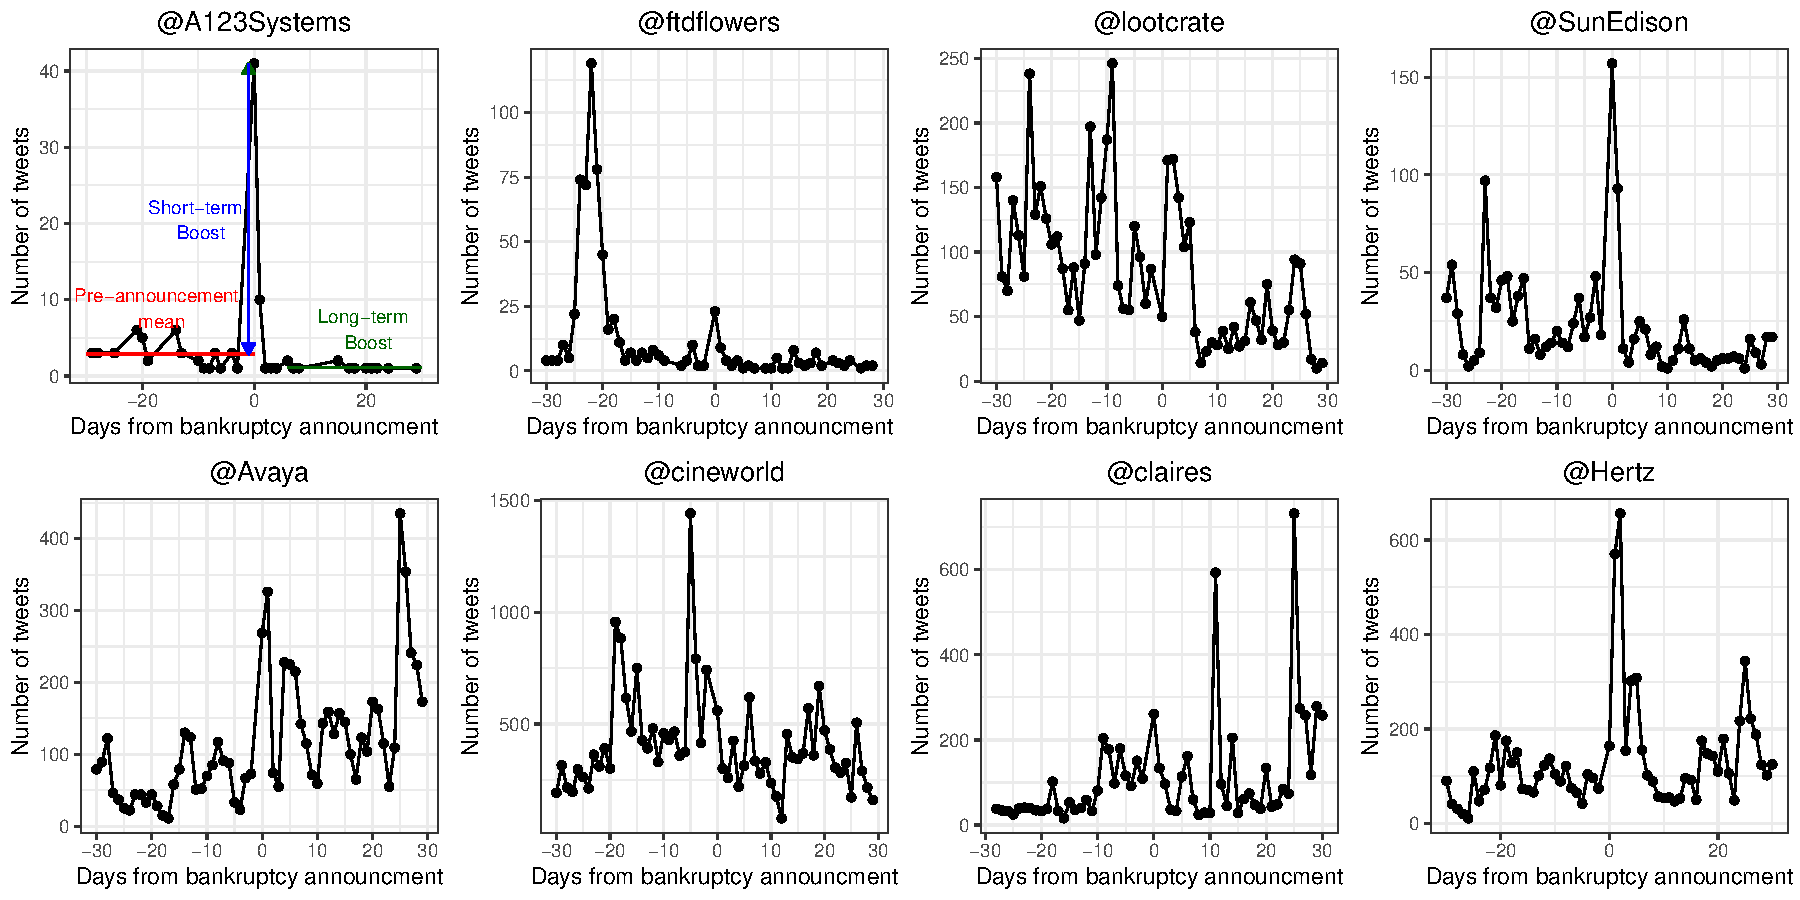
\includegraphics[scale=.5,trim={0cm 0cm 0cm 0cm},clip]{images/spikes.pdf}
    \caption{ 
            Examples of mention time series for 8 companies, as recorded from Twitter posts (tweets).
            Companies' Twitter handles begin with `@' above each figure.
            Companies in the top row experienced a rapid increase followed by a quick decay in attention after bankruptcy announcement at $t_0$.
            Companies in the bottom row also experienced a rapid increase in attention following bankruptcy, but attention was more persistent (decreased more slowly) compared with companies in the top row in terms of days until returning to pre-announcement mean.
            From each mention time series, we extract three characteristic values (illustrated in the top left figure): Pre-Announcement Mean (PAM), Short-Term Boost, and Long-Term Boost, as defined in Table \ref{tbl:def}.
            }
    \label{fig:spikes}
\end{figure*}


\newpage

\begin{figure}[h!]
\center
    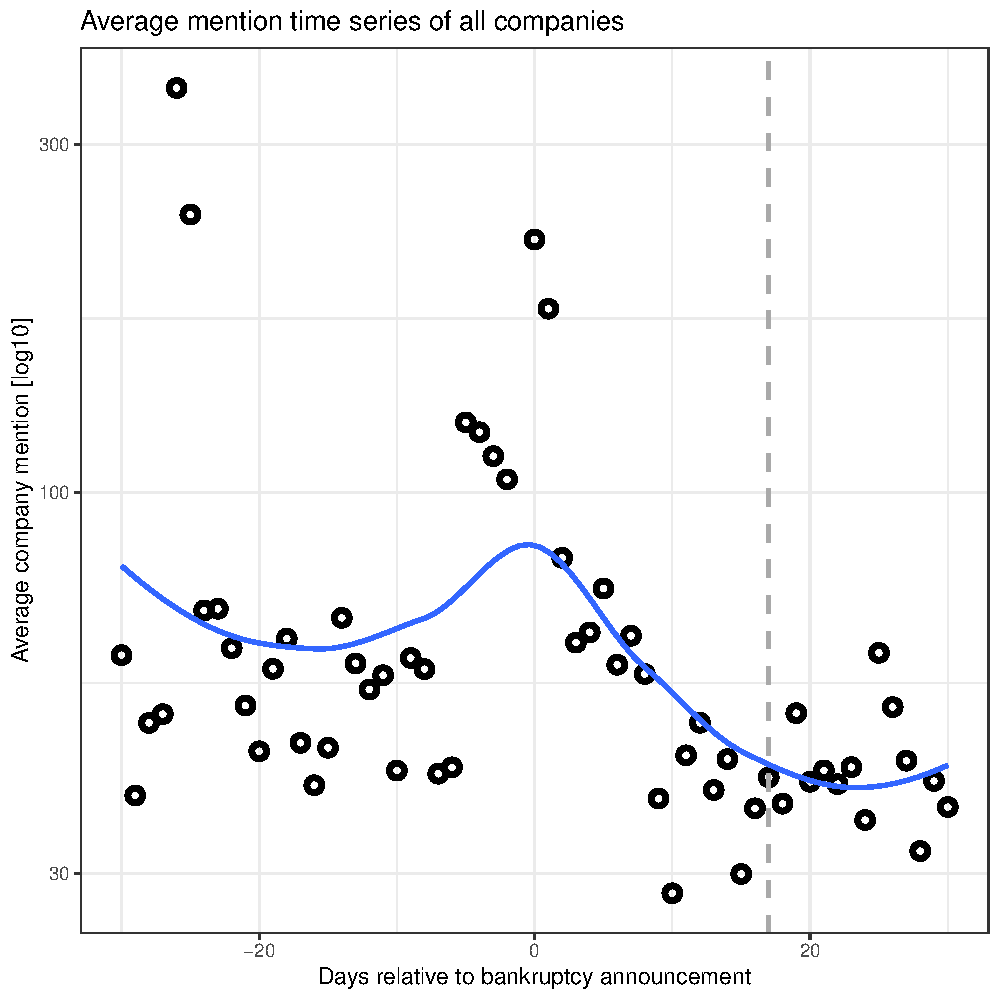
\includegraphics[scale=.5,trim={0cm 0cm 0cm 0.6cm},clip]{images/mean_curve.pdf}
    \caption{ 
           Average company mention time series of the 74 companies included in the study (see Fig. \ref{fig:spikes} for examples of individual mention time series). 
            The average was obtained via the arithmetic mean of the individual raw mention time series of companies that declared bankruptcy.
            The average mention frequency value spikes at the day of bankruptcy announcement ($t_0$) and fades quickly after $t_I=17$ days (vertical dashed line).
            Inflection Point $t_I$ denotes the maximum curvature cutoff point for $t>0$.
            Circles correspond to raw average mention time series, and the blue curve, to the mean smoothed version.
            }
    \label{fig:mean_curve}
\end{figure}

\newpage

\begin{figure*}[htbp]
  \centering
  \begin{subfigure}[b]{0.45\textwidth}
    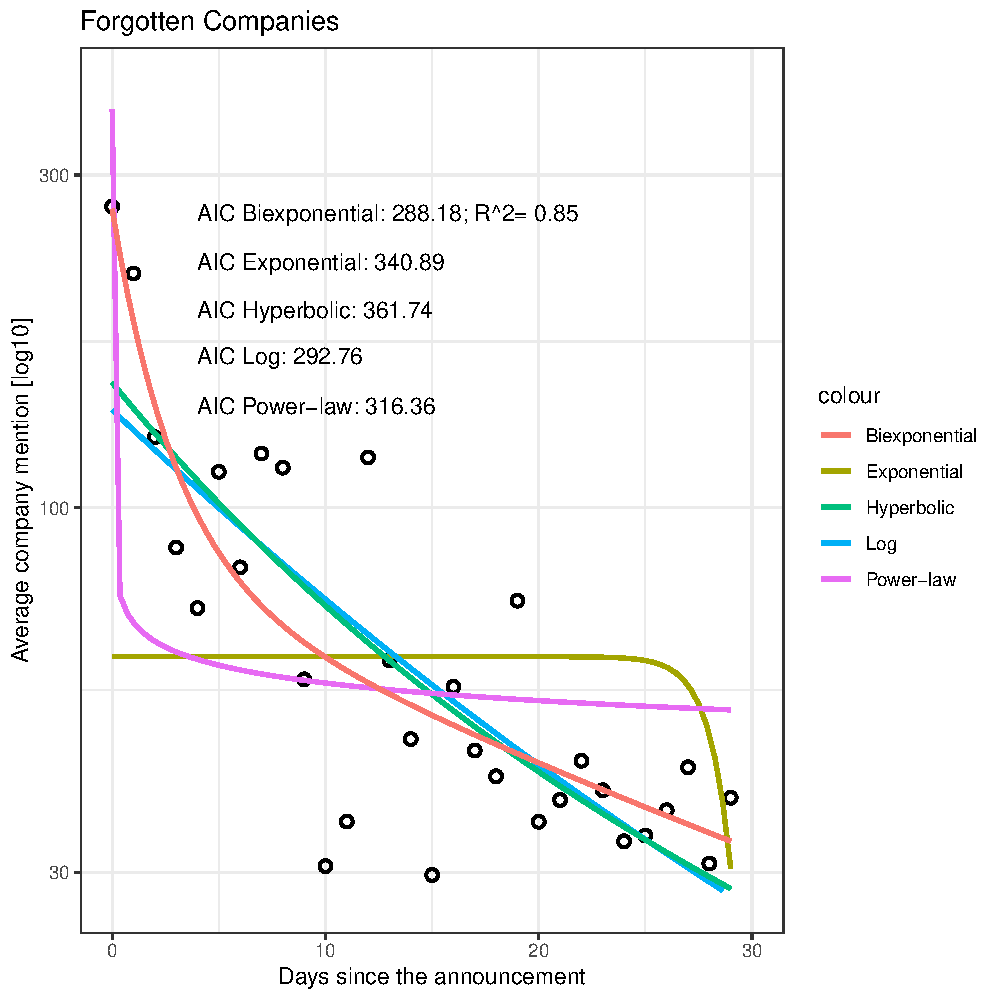
\includegraphics[scale=.5,trim={0cm 0cm 3.5cm 0.7cm},clip]{images/forgotten_models.pdf}
    \caption{Low persistence.}
    \label{fig:sub1}
  \end{subfigure}
  \hfill
  \begin{subfigure}[b]{0.45\textwidth}
    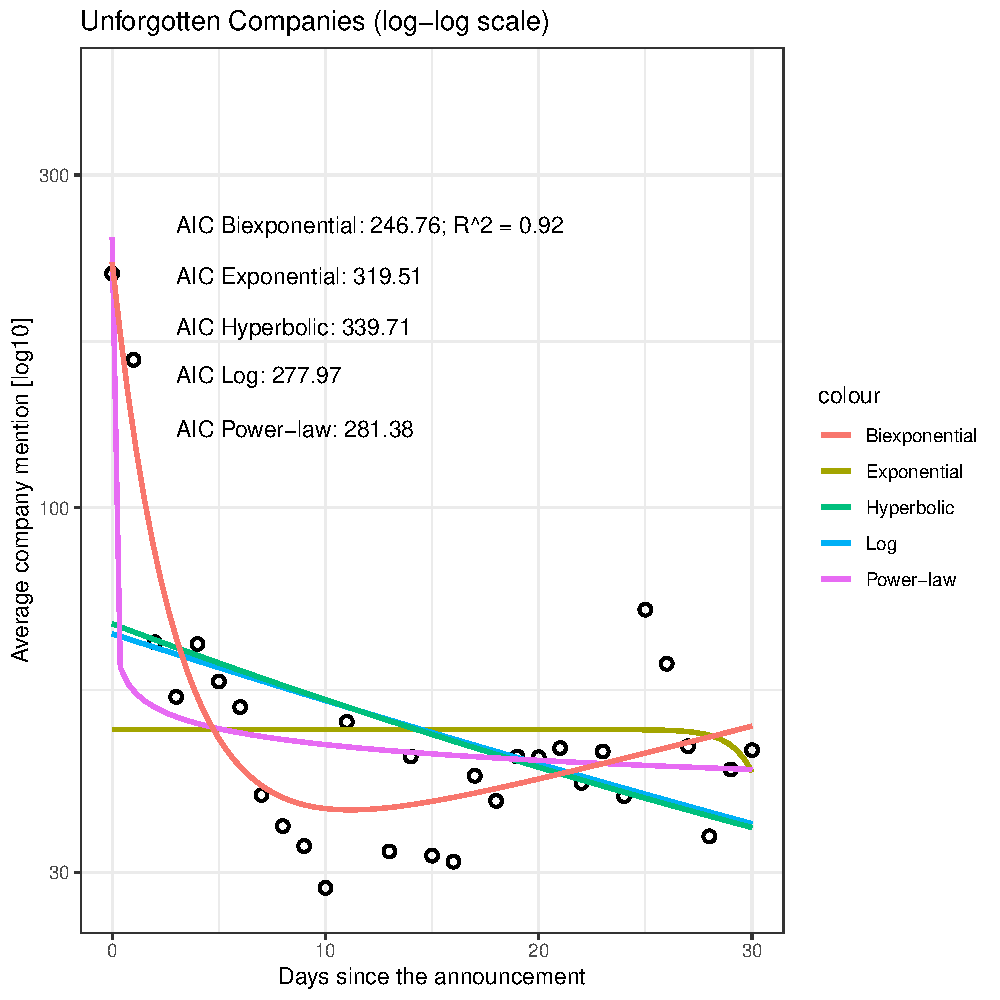
\includegraphics[scale=.5,trim={0cm 0cm 0cm 0.7cm},clip]{images/Unforgotten_models.pdf}
    \caption{High persistence.}
    \label{fig:sub2}
  \end{subfigure}
  \caption{
            Model fitting for bankruptcy events of Low and High memory persistence.
            Higher $R^2$ and lower AIC values indicate a better fit.
  }
  \label{fig:models}
\end{figure*}


\newpage

\begin{figure}[h!]
\center
    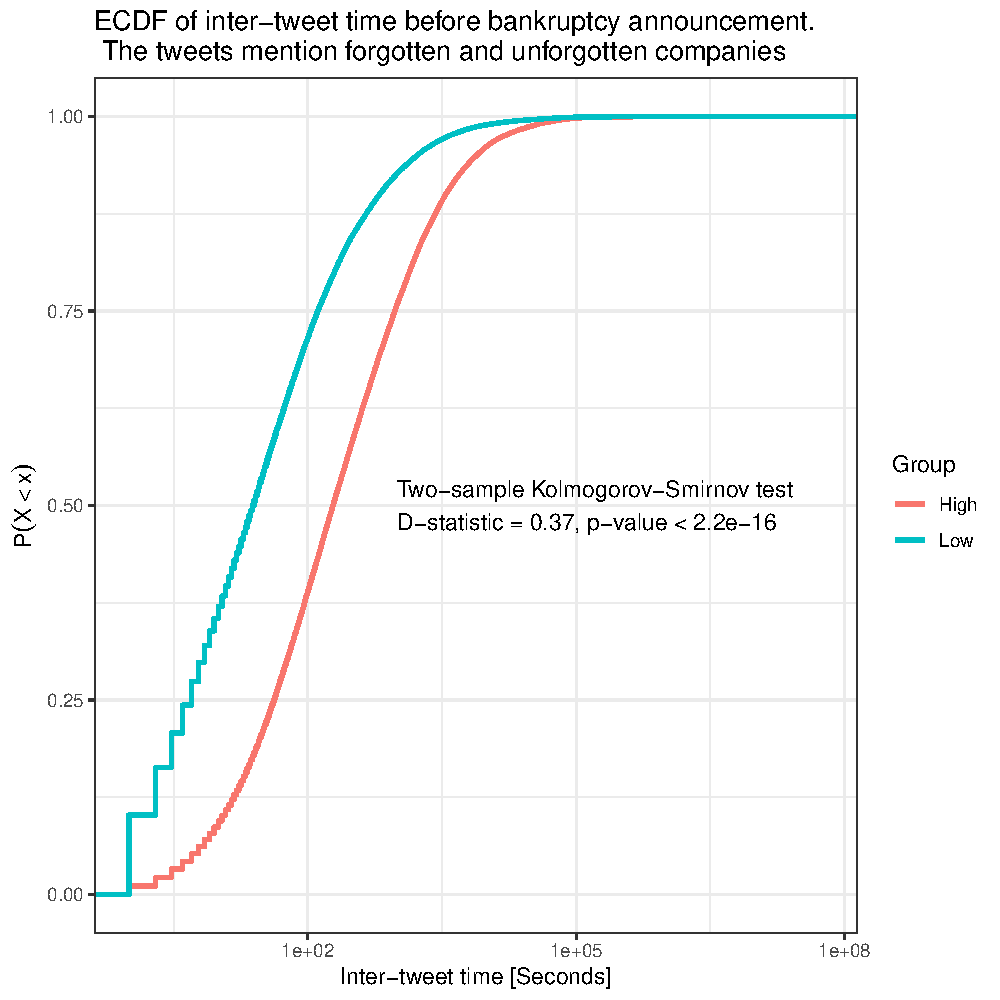
\includegraphics[scale=.5,trim={0cm 0cm 0cm 1.2cm},clip]{images/ecdf.pdf}
    \caption{ 
           Empirical Cumulative Distribution Function (ECDF) of inter-tweet time before bankruptcy announcement for Low and High persistent memory of bankruptcy events.
           High and Low persistent memory have different temporal tweeting patterns, identified via comparison of the two ECDFs by using the Kolmogorov-Smirnov test.
           P-value < 0.05 indicates that the samples are not drawn from the same distribution.
            }
    \label{fig:ecdf}
\end{figure}


\newpage

\begin{table*}[h!]
\centering
\caption{Definitions of variables}
\label{tbl:def}
\begin{tabular}{llll}
Parameter         & Definition      & Mathematical Definition                                            &  \\ \cline{1-3}
\begin{tabular}[c]{@{}l@{}}
Bankruptcy event start
\end{tabular} 
& Day of bankruptcy announcement.                                                                                                   & $t_0$                                              &  \\
\begin{tabular}[l]{@{}l@{}}
Studied attention period
\end{tabular} 
& Time period (days) before and after bankruptcy announcement.                                                              & $t \in [t_0 - \Delta t, t_0 + \Delta t]$                           &  \\
\begin{tabular}[l]{@{}l@{}}
Pre-Announcement\\Mean (PAM)
\end{tabular} & 
\begin{tabular}[l]{@{}l@{}}
Mean daily mentions before bankruptcy announcement.
\end{tabular} 
& $Mean(\{mentions_t | t < t_0\})$            &  \\
\begin{tabular}[l]{@{}l@{}}
Inflection Point ($t_I$) 
\end{tabular} 
& 
\begin{tabular}[l]{@{}l@{}}
Point in time when communicative memory shifts into\\ an extended, flatter phase.   
\end{tabular} 
& $\{t_I | mentions_{t_I} \le PAM, t_I > t_0\}$                                        &  \\
\begin{tabular}[l]{@{}l@{}}
Short-Term   
\end{tabular} 
& Time period (days) between bankruptcy announcement and $t_I$.                                                                 & $t \in [t_0, t_I]$                                 &  \\
\begin{tabular}[l]{@{}l@{}}
Long-Term
\end{tabular} 
& Time period (days) after $t_I$.                                                                                               & $t > t_I$                                  &  \\
\begin{tabular}[l]{@{}l@{}}
Short-Term Boost   
\end{tabular} 
& Maximum daily mentions in the Short-Term period minus PAM.                                                                        & $Max(\{mentions_t | t \in [t_0,t_I]\}) - PAM$      &  \\
\begin{tabular}[l]{@{}l@{}}
Long-Term Boost      
\end{tabular} 
& \begin{tabular}[l]{@{}l@{}}
Mean daily mentions after the Inflection Point minus PAM.\end{tabular}  & $Mean(\{mentions_t | t > t_I\}) - PAM$     &  \\
\begin{tabular}[l]{@{}l@{}}Persistence\\ Level of Memory \end{tabular}                                                   & \begin{tabular}[l]{@{}l@{}}
Maximum daily mentions in the Long-term period compared\\ with PAM.
\end{tabular}          & 
\begin{tabular}[l]{@{}l@{}}

    $High:$ \textit{if} $Max\{mentions_t \mid t > t_I\} > PAM$ \\
    $Low:$ $otherwise$

\end{tabular}
&
 \\ \cline{1-3}
\end{tabular}
\end{table*}

\end{document}

